% -----------------------------------------------------------------------------
\section{Purpose}
% -----------------------------------------------------------------------------

Synthetic biology builds upon the techniques and successes of genetics, molecular biology, and metabolic engineering by applying engineering principles to the design of biological systems. 
When designing a synthetic system, synthetic biologists need to exchange information about multiple types of molecules and their expected/actual behavior.
Furthermore, there are often multiple aspects to a design such as a specified nucleic acid sequence (e.g. a sequence that encodes an enzyme or transcription factor), the molecular interactions that a designer intends to result from the introduction of the said sequence (e.g., chemical modification of metabolites or regulation of gene expression), and the experiments and data associated with the system. Yet all these perspectives need to be connected together in the engineering of biological systems.

The \emph{Synthetic Biology Open Language} (SBOL) has been developed as a standard to support the specification and exchange of biological design information in synthetic biology, 
following an open community process involving both ``wet'' bench scientists and ``dry'' scientific modelers and software developers across academia, industry, and other institutions.
Previous nucleic acid sequence description formats lack key capabilities relative to SBOL, as shown in \ref{f:sequence}. 
Simple sequence encoding formats such as FASTA encode little besides sequence information. 
More sophisticated formats such as GenBank and Swiss-Prot provide a flat annotation of sequence features well suited to description of natural systems, but unable to represent the functional relations and multi-layered design structure common to engineered systems.
Modeling languages, such as the Systems Biology Markup Language (SBML) ~\cite{SBML} can be used represent biological processes, but are not sufficient to represent the associated nucleotide or amino acid sequences.  
SBOL covers both of these needs, representing both the structure and function of a genetic design in a modular, hierarchical manner, as well as its relationship to and use within experiment plans, data, models, etc.

\begin{figure}[htbp!]
\centering
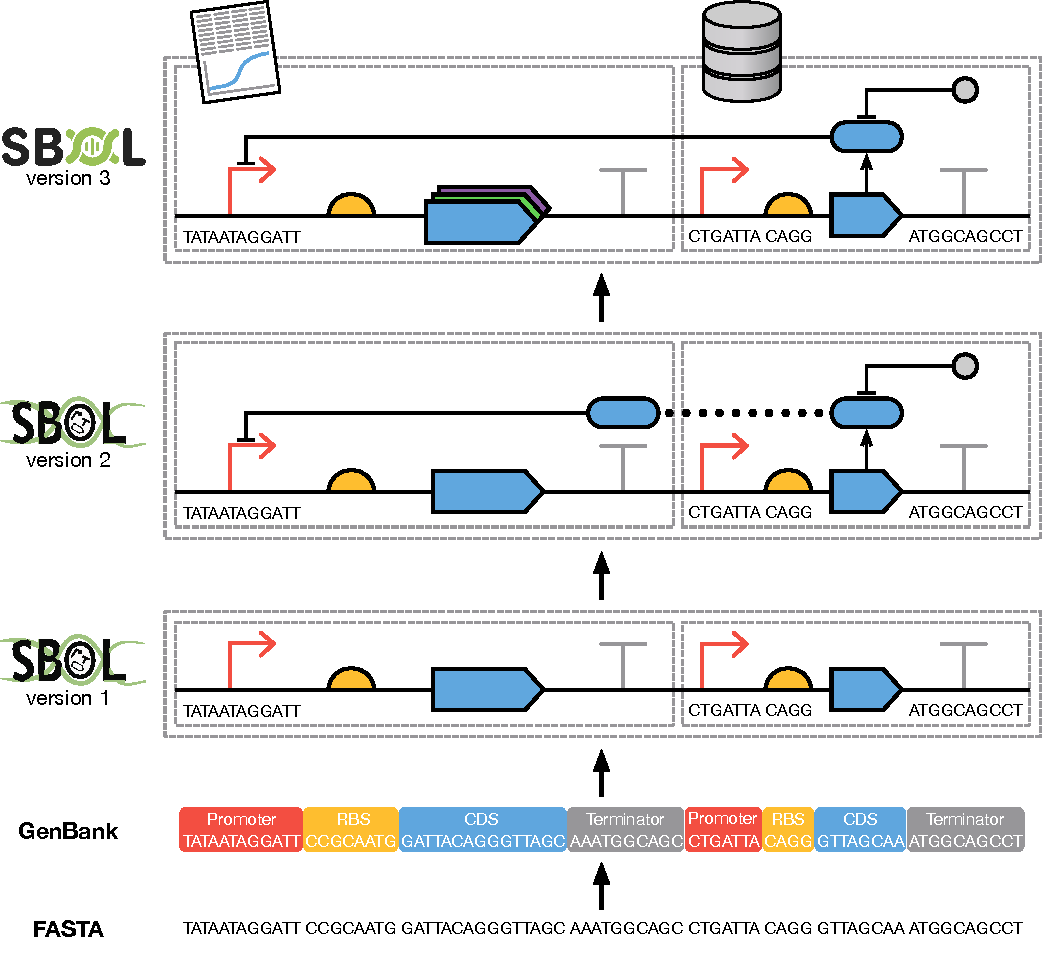
\includegraphics[width=0.8\textwidth]{images/SBOL3-evolution.pdf}
\caption{SBOL extends prior sequence description formats to represent both the structure and function of a genetic design in a modular, hierarchical manner, as well as its relationship to, and use within, experiments, plans, data, models, etc.}
\label{f:sequence}
\end{figure}

SBOL uses existing Semantic Web practices and resources, such as \emph{Uniform Resource Identifiers} (\sbol{URI}s) and ontologies, to unambiguously identify and define biological system elements,
and to provide serialization formats for encoding this information in electronic data files.
The SBOL standard further describes the rules and best practices on how to use this data model and populate it with relevant design details. 
The definition of the data model, the rules on the addition of data within the format, and the representation of this in electronic data files are intended to make the SBOL standard a useful means of promoting data exchange between laboratories and between software programs.

\subsection{Differences from Prior Versions of SBOL}
SBOL 1 focused on representing the structural aspects of genetic designs. Users of the standard were able to exchange information on DNA designs, but they could not represent molecules other than DNA or the functional aspects of designs beyond DNA sequence features. SBOL 2 enabled the description and exchange of hierarchical, modular representations of both the intended structure and function of designed biological systems, as well as support for representing provenance, combinatorial designs, genetic design implementations, external file attachments, experimental data, and numerical measurements. 
SBOL 3, detailed in this document, now condenses and simplifies these prior representations based on experiences in deployment across a variety of scientific and industrial settings.

This document details version 3.0 of SBOL.  
In particular, SBOL 3.0 includes the following changes relative to the prior SBOL 2.3:
\begin{itemize}
\item Separation of sequence features from part/sub-part relationships.
\item ComponentDefinition/Component is renamed to Component/SubComponent.
\item Merges Component and Module classes.
\item Ensures consistency between data model and ontology terms.
\item Extends the means to define and reference SubComponents.
\item Refines requirements on object URIs.
\item Enables graph-based serialization.
\item Moves to Systems Biology Ontology (SBO) for Component types.
\item Makes all sequence associations explicit.
\item Makes interfaces explicit.
\item Generalizes SequenceConstraints into a general structural Constraint class.
\item Expands the set of allowed sequence constraints.
\end{itemize}

